\documentclass[../main/report.tex]{subfiles}
\begin{document}

\section{Backup oriented design}

When designing a system, the PCB is one of the harder things to debug.
If a wire inside the PCB is wrong, there is not much that can be done, except buying a new PCB.
This becomes apparent when seeing most projects only have a working PCB on the 3rd of maybe even the 4th try. \todo{Citation needed}
Because of this, a strong philosophy of backup plans has been used in the design for the PCB.

\begin{figure}[H]
    \centering
    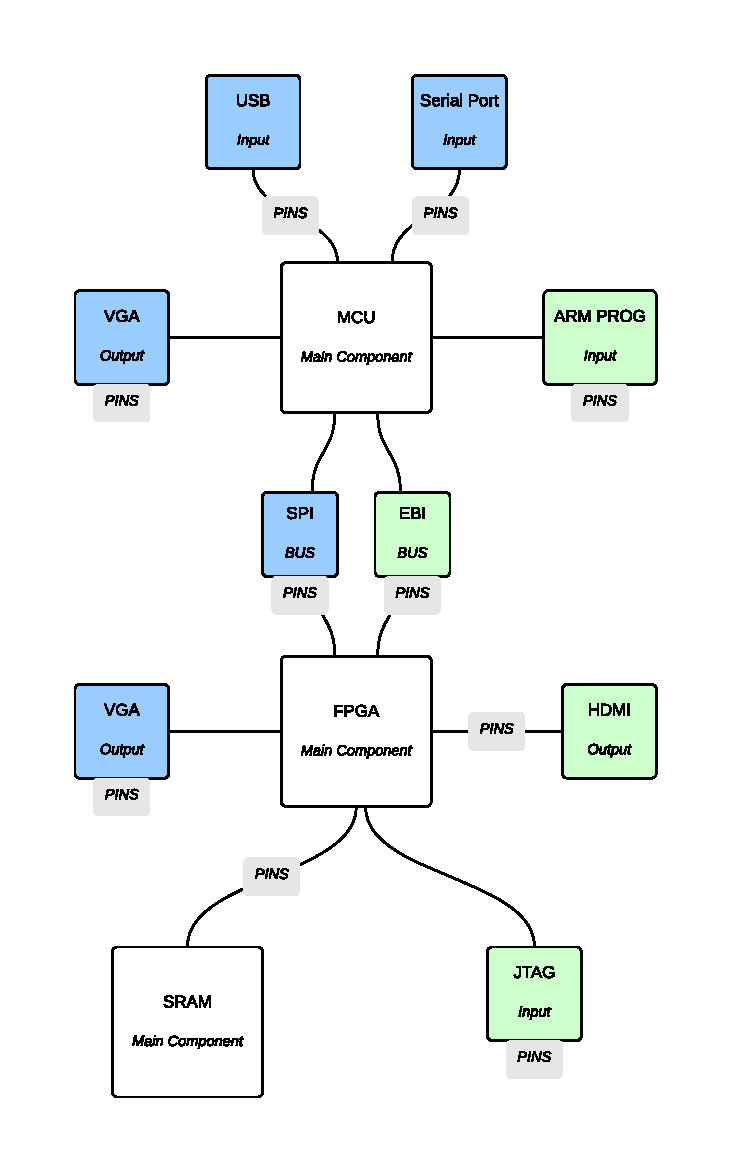
\includegraphics[width=0.65\textwidth]{../pcb/assets/pcb-overview.pdf}
    \label{fig:pcb-overview}
    \caption{Conceptual overview of the PCB. Green boxes are main solutions. Blue boxes are backup plans.
             Gray boxes labeled "PINS" means there are pins either on the wire itself, or that the box is pins.}
\end{figure}

These backup plans are in place to make sure the board will work, even if some parts are broken.
All important wires and unused pins have been put onto headers, which can be rerouted manually.
That way, each component can be connected to other sources than that on the board alone.
Because of this, the board is not optimized for the smallest size possible, but was rather made to optimize for highest possible chance of success.

\end{document}
